\subsection{SP3: juego distribuido de contactos y factibilidad \emph{wrench}}
\label{sec:resultados-sp3}

\subsubsection{Frontera respecto de SP2}

SP2 responde cuánta capacidad efectiva recibe una carga. SP3 pregunta si esa
capacidad, aplicada desde contactos concretos, puede producir la fuerza y el momento
requeridos. La decisión deja de ser robot--carga y pasa a ser
robot--carga--slot--fuerza. Esta distinción pertenece al espacio de \emph{wrenches} y
de cierre por fuerzas: sumar capacidades escalares no caracteriza las direcciones ni
los momentos realizables por un conjunto de contactos
\citep{ferrari1992grasps,bicchi1995closure}.

Para la carga planar $k$, sea
$q_k=[p_{x,k},p_{y,k},\theta_k]^\top$. El wrench comandado en un instante se obtiene
del modelo de Euler--Lagrange,
\[
 w_k^{\rm dem}
 =M_k(q_k)\ddot q_k^{\rm ref}
 +C_k(q_k,\dot q_k)\dot q_k+d_k(q_k,\dot q_k),
 \qquad
 w_k^{\rm dem}=[F_{x,k},F_{y,k},\tau_{z,k}]^\top .
\]
SP3 usa esta demanda como fotografía cuasiestática. Integrar la pose, seguir una
trayectoria y evitar obstáculos corresponde a SP4--SP5.

Un slot $s$ tiene posición relativa $r_{ks}=[r_x,r_y]^\top$ y dirección unilateral
$d_{ks}=[d_x,d_y]^\top$. Una magnitud de fuerza $\varphi_{iks}\geq0$ produce
\[
 g_{ks}\varphi_{iks},\qquad
 g_{ks}=
 \begin{bmatrix}
 d_x & d_y & r_xd_y-r_yd_x
 \end{bmatrix}^{\!\top}.
\]
Para una selección $C_k$, el ajuste mecánico interno es
\[
 \rho_k(C_k)=
 \min_{0\leq\varphi_{iks}\leq\bar f_i}
 \left\|D_w^{-1}
 \left(w_k^{\rm dem}-\sum_{(i,s)\in C_k}g_{ks}\varphi_{iks}\right)
 \right\|_2 ,
 \quad D_w=\operatorname{diag}(F_{\rm ref},F_{\rm ref},\tau_{\rm ref}).
 \label{eq:sp3-rho}
\]
La carga supera la comprobación cuando $\rho_k\leq\varepsilon_w$ y no existen conflictos
de slots.

\begin{proposicion}[La capacidad escalar no es suficiente]
Existe una coalición que satisface la demanda escalar de SP2 y no puede satisfacer
\eqref{eq:sp3-rho}.
\end{proposicion}
\begin{proof}
Considérese una demanda de torque puro y dos robots cuya capacidad total excede la
demanda escalar. Si ambos empujan en la misma línea de acción, el torque resultante
es cero. En cambio, dos fuerzas opuestas en slots separados forman el par requerido.
La capacidad total coincide en ambos casos, pero el conjunto de wrenches realizables
es distinto.
\end{proof}

Con $C_k$ fijo, \eqref{eq:sp3-rho} es un problema convexo de mínimos cuadrados
acotados. La selección conjunta sigue siendo NP-hard porque al hacer coincidir todos
los slots y direcciones se recupera el cierre heterogéneo de SP2. El coste polinomial
del ajuste interior no elimina la dificultad combinatoria exterior.

\subsubsection{Relajación convexa y juego con restricciones compartidas}

Sea $\mathcal A$ el conjunto de pares carga--slot y
$x_i\in\Delta^{|\mathcal A|+1}$ la utilización fraccional del robot $i$, incluida la
estrategia de reposo. La columna normalizada de la acción $(k,s)$ es
$h_{iks}=\bar f_iD_w^{-1}g_{ks}$ y
$\widetilde w_k=D_w^{-1}w_k^{\rm dem}$. Se propone el potencial
\[
 \Phi(x)=
 -\frac12\sum_k
 \left\|\widetilde w_k-\sum_{i,s}h_{iks}x_{iks}\right\|_2^2
 -\sum_{i,k,s}c_{iks}x_{iks}
 -\frac{\epsilon}{2}\sum_{i,k,s}x_{iks}^2 ,
 \label{eq:sp3-potential}
\]
sujeto a ocupación compartida
$\sum_i x_{iks}\leq1$. El coste $c_{iks}$ representa desplazamiento y
$\epsilon>0$ regulariza el reparto.

La forma primal introduce
$r_k=\widetilde w_k-\sum_{i,s}h_{iks}x_{iks}$ y minimiza $-\Phi$. Con
$\lambda_k$ para la igualdad wrench y $\mu_{ks}\geq0$ para cada slot,
\[
 \mathcal L=
 \frac12\sum_k\norm{r_k}^2+c^\top x+\frac{\epsilon}{2}\norm{x}^2
 +\sum_k\lambda_k^\top(\widetilde w_k-H_kx-r_k)
 +\mu^\top(Bx-\mathbf1).
\]
Las condiciones KKT relevantes son
\[
 \lambda_k=r_k,\qquad
 0\in c+\epsilon x-H^\top\lambda+B^\top\mu+N_{\Delta}(x),
 \qquad
 0\leq\mu\perp\mathbf1-Bx\geq0 .
 \label{eq:sp3-kkt}
\]
Así, el residual de fuerza y torque es también un precio vectorial: una acción recibe
valor cuando su columna $h_{iks}$ está alineada con $\lambda_k$.

\begin{proposicion}[KKT y equilibrio variacional]
Si los conjuntos locales son convexos, existe un punto de Slater y $\epsilon>0$, las
KKT de \eqref{eq:sp3-kkt} son necesarias y suficientes para el óptimo de la relajación.
Ese punto coincide con el v-GNE del juego de potencial con multiplicador compartido.
\end{proposicion}
\begin{proof}
El negativo de \eqref{eq:sp3-potential} es convexo y diferenciable; las restricciones
son afines y los simplex son convexos y compactos. Slater da suficiencia de KKT. El
pseudogradiente de cada jugador coincide con el bloque correspondiente del gradiente
del potencial. Compartir el multiplicador de la restricción acoplada produce la
desigualdad variacional de un v-GNE.
\end{proof}
Esta equivalencia es estándar para juegos convexos con restricciones compartidas y
algoritmos primal--dual distribuidos \citep{yi2019operator,cherukuri2016primaldual}.
No se extiende al cierre entero.

\begin{figure}[H]
\centering
\begin{tikzpicture}[
  node distance=10mm and 13mm,
  state/.style={draw=VIULinkBlue, rounded corners=1.5mm, fill=VIULight,
    minimum width=34mm, minimum height=13mm, align=center, font=\small},
  dual/.style={state, draw=VIUOrange, fill=VIUOrange!10},
  flow/.style={->, >=stealth, thick, draw=VIUDeep}
]
\node[state] (primal) {Primal\\$x_{iks}$};
\node[dual, right=of primal] (wrench) {Precio wrench\\$\lambda_k=r_k$};
\node[dual, below=of wrench] (slot) {Precio de slot\\$\mu_{ks}\geq0$};
\node[state, left=of slot] (equilibrium) {v-GNE / KKT\\relajación convexa};

\draw[flow] (primal) -- node[above, font=\scriptsize] {$\widetilde w-Hx$} (wrench);
\draw[flow] (wrench) -- node[right, font=\scriptsize] {$H^\top\lambda$} (slot);
\draw[flow] (slot) -- node[below, font=\scriptsize] {complementariedad} (equilibrium);
\draw[flow] (equilibrium) -- node[left, font=\scriptsize] {proyección} (primal);
\draw[flow, dashed] (primal) -- node[below, font=\scriptsize] {$Bx-\mathbf1$} (slot);
\end{tikzpicture}
\caption[Relación entre primal--dual, KKT y v-GNE]{El residual wrench actúa como precio vectorial; los multiplicadores de slot imponen la restricción compartida. La equivalencia se limita a la relajación convexa.}
\viuownsource
\label{fig:sp3-kkt-game}
\end{figure}


\subsubsection{Primal--dual, population dynamics y Nash seeking}

El payoff común para cualquier motor de revisión es
\[
 \pi_{iks}=h_{iks}^{\top}\lambda_k-c_{iks}-\epsilon x_{iks}-\mu_{ks},
 \qquad \lambda_k=\widetilde w_k-\sum_{i,s}h_{iks}x_{iks}.
 \label{eq:sp3-payoff}
\]
El método con contrato KKT usa ascenso proyectado en cada simplex y ascenso dual:
\[
 \dot x_i=\Pi_{T_{\Delta}(x_i)}[\pi_i],
 \qquad
 \dot\mu=[Bx-\mathbf1]^+_{\mu}.
 \label{eq:sp3-pd}
\]
Bajo las hipótesis anteriores, estas dinámicas de punto silla convergen al conjunto
primal--dual \citep{cherukuri2016primaldual}. La implementación usa Euler proyectado;
una referencia SLSQP independiente resuelve el mismo QP.

Como ablación del motor, el mismo payoff alimenta Smith, replicator y ERV--BNN:
\[
 \dot x_{ia}^{\rm rep}=x_{ia}(\pi_{ia}-\bar\pi_i),\qquad
 \dot x_{ia}^{\rm BNN}=[\pi_{ia}-\bar\pi_i]_+
 -x_{ia}\sum_b[\pi_{ib}-\bar\pi_i]_+ ,
\]
mientras Smith intercambia masa mediante ventajas positivas entre pares. Los tres
campos conservan el simplex; no se les transfiere automáticamente el teorema KKT del
projected primal--dual.

Con información parcial, cada robot estima la contribución wrench y la ocupación de
slots mediante consenso. Cuatro rondas Metropolis sobre un anillo producen
$\widehat\lambda_{ik}$ y $\widehat\mu_{iks}$ para \eqref{eq:sp3-payoff}. Esta estructura
sigue el principio de juegos agregativos sobre grafos y GNE con información parcial
\citep{koshal2016aggregative,yi2019operator,franci2022stochasticgne}. En este TFM,
el grafo completo representa información exacta; el anillo es una sensibilidad
numérica y no un teorema para topologías variables.

Para $A=|\mathcal A|$, projected primal--dual, replicator y BNN cuestan
$O(NA)$ por iteración; Smith cuesta $O(NA^2)$ y $R$ rondas de consenso
$O(R|E|(3K+A))$. Estos costes no acotan las iteraciones ni resuelven el problema
entero NP-hard.

\begin{figure}[H]
\centering
\begin{tikzpicture}[
  node distance=6mm and 7mm,
  box/.style={draw=VIULinkBlue, rounded corners=1.5mm, fill=VIULight,
    minimum width=29mm, minimum height=12mm, align=center, font=\small},
  phys/.style={box, draw=VIUOrange, fill=VIUOrange!10},
  guard/.style={box, draw=VIUDeep, fill=VIUDeep!8},
  flow/.style={->, >=stealth, thick, draw=VIUDeep}
]
\node[phys] (dynamics) {Euler--Lagrange\\$w_k^{\rm dem}$};
\node[phys, right=of dynamics] (contacts) {Slots y matriz\\$g_{ks}$};
\node[box, right=of contacts] (estimate) {Nash seeking\\$\widehat w_{ik},\widehat y_{iks}$};
\node[box, right=of estimate] (prices) {Precios\\$\lambda_k,\mu_{ks}$};

\node[box, below=of prices] (revision) {Revisión\\PD / Smith /\\replicator / BNN};
\node[box, left=of revision] (raw) {Preferencia RAW\\$x_i\in\Delta^{A+1}$};
\node[guard, left=of raw] (closure) {Cierre entero\\robot--carga--slot};
\node[guard, left=of closure] (certificate) {Guardia wrench\\$\rho_k\leq\varepsilon_w$};

\draw[flow] (dynamics) -- (contacts);
\draw[flow] (contacts) -- (estimate);
\draw[flow] (estimate) -- (prices);
\draw[flow] (prices) -- (revision);
\draw[flow] (revision) -- (raw);
\draw[flow] (raw) -- (closure);
\draw[flow] (closure) -- (certificate);
\draw[flow, dashed] (certificate.north) to[bend left=18]
  node[above, font=\scriptsize, align=center]{residual y abstención} (estimate.south);
\end{tikzpicture}
\caption[Arquitectura del juego wrench de SP3]{SP3 separa demanda dinámica, geometría de contacto, estimación agregada, revisión continua, cierre entero y comprobación mecánica dentro del modelo.}
\viuownsource
\label{fig:sp3-wrench-nash-architecture}
\end{figure}


\subsubsection{Cierre entero y contrato de seguridad}

RAW toma el argmax de cada $x_i$ y puede repetir slots. El cierre de slots resuelve
conflictos por preferencia. La guardia añade robots individualmente o por pares,
recalcula \eqref{eq:sp3-rho} y elimina incondicionalmente toda carga con
$\rho_k>\varepsilon_w$. Por construcción, una carga CLOSED aceptada no es falso
positivo respecto del modelo implementado.

La guardia observa preferencias, todos los robots libres, geometría completa y el
solver de wrench. Por ello se declara global, no plenamente distribuida. Su función
es comprobar y medir la brecha entre equilibrio continuo y decisión ejecutable, no
demostrar que el sistema extremo a extremo esté descentralizado.

\subsubsection{Diseño experimental y validaciones}

La campaña canónica \texttt{SP3\_WRENCH\_NASH\_GAME\_v1\_1} usa seis familias:
punto degenerado, torque puro, empuje unilateral, centro de masa excéntrico, carga
larga y saturación de slots. Cien semillas nuevas por familia producen 600 mundos y
7200 ejecuciones. Los doce métodos incluyen oráculos wrench/escalar, CBBA, greedy
wrench, cierre pareado, uniforme+guardia, projected primal--dual exacto y en anillo,
y Smith, replicator y ERV--BNN con el mismo precio.

La métrica primaria es el falso positivo condicionado a asignación. Se añaden
cobertura respecto del oráculo, precisión, residual, brecha, KKT, mensajes y tiempo.
Los cuatro contrastes se congelaron antes de v1.1, son pareados por mundo, usan
bootstrap del 95\,\%, Wilcoxon unilateral y Holm. La v1 original se conserva como
no canónica: con 500 iteraciones excedió el gate QP de $0{,}01$. v1.1 modificó solo
el horizonte projected primal--dual a 1200 y abrió semillas 461000--461099.

\begin{figure}[H]
\centering
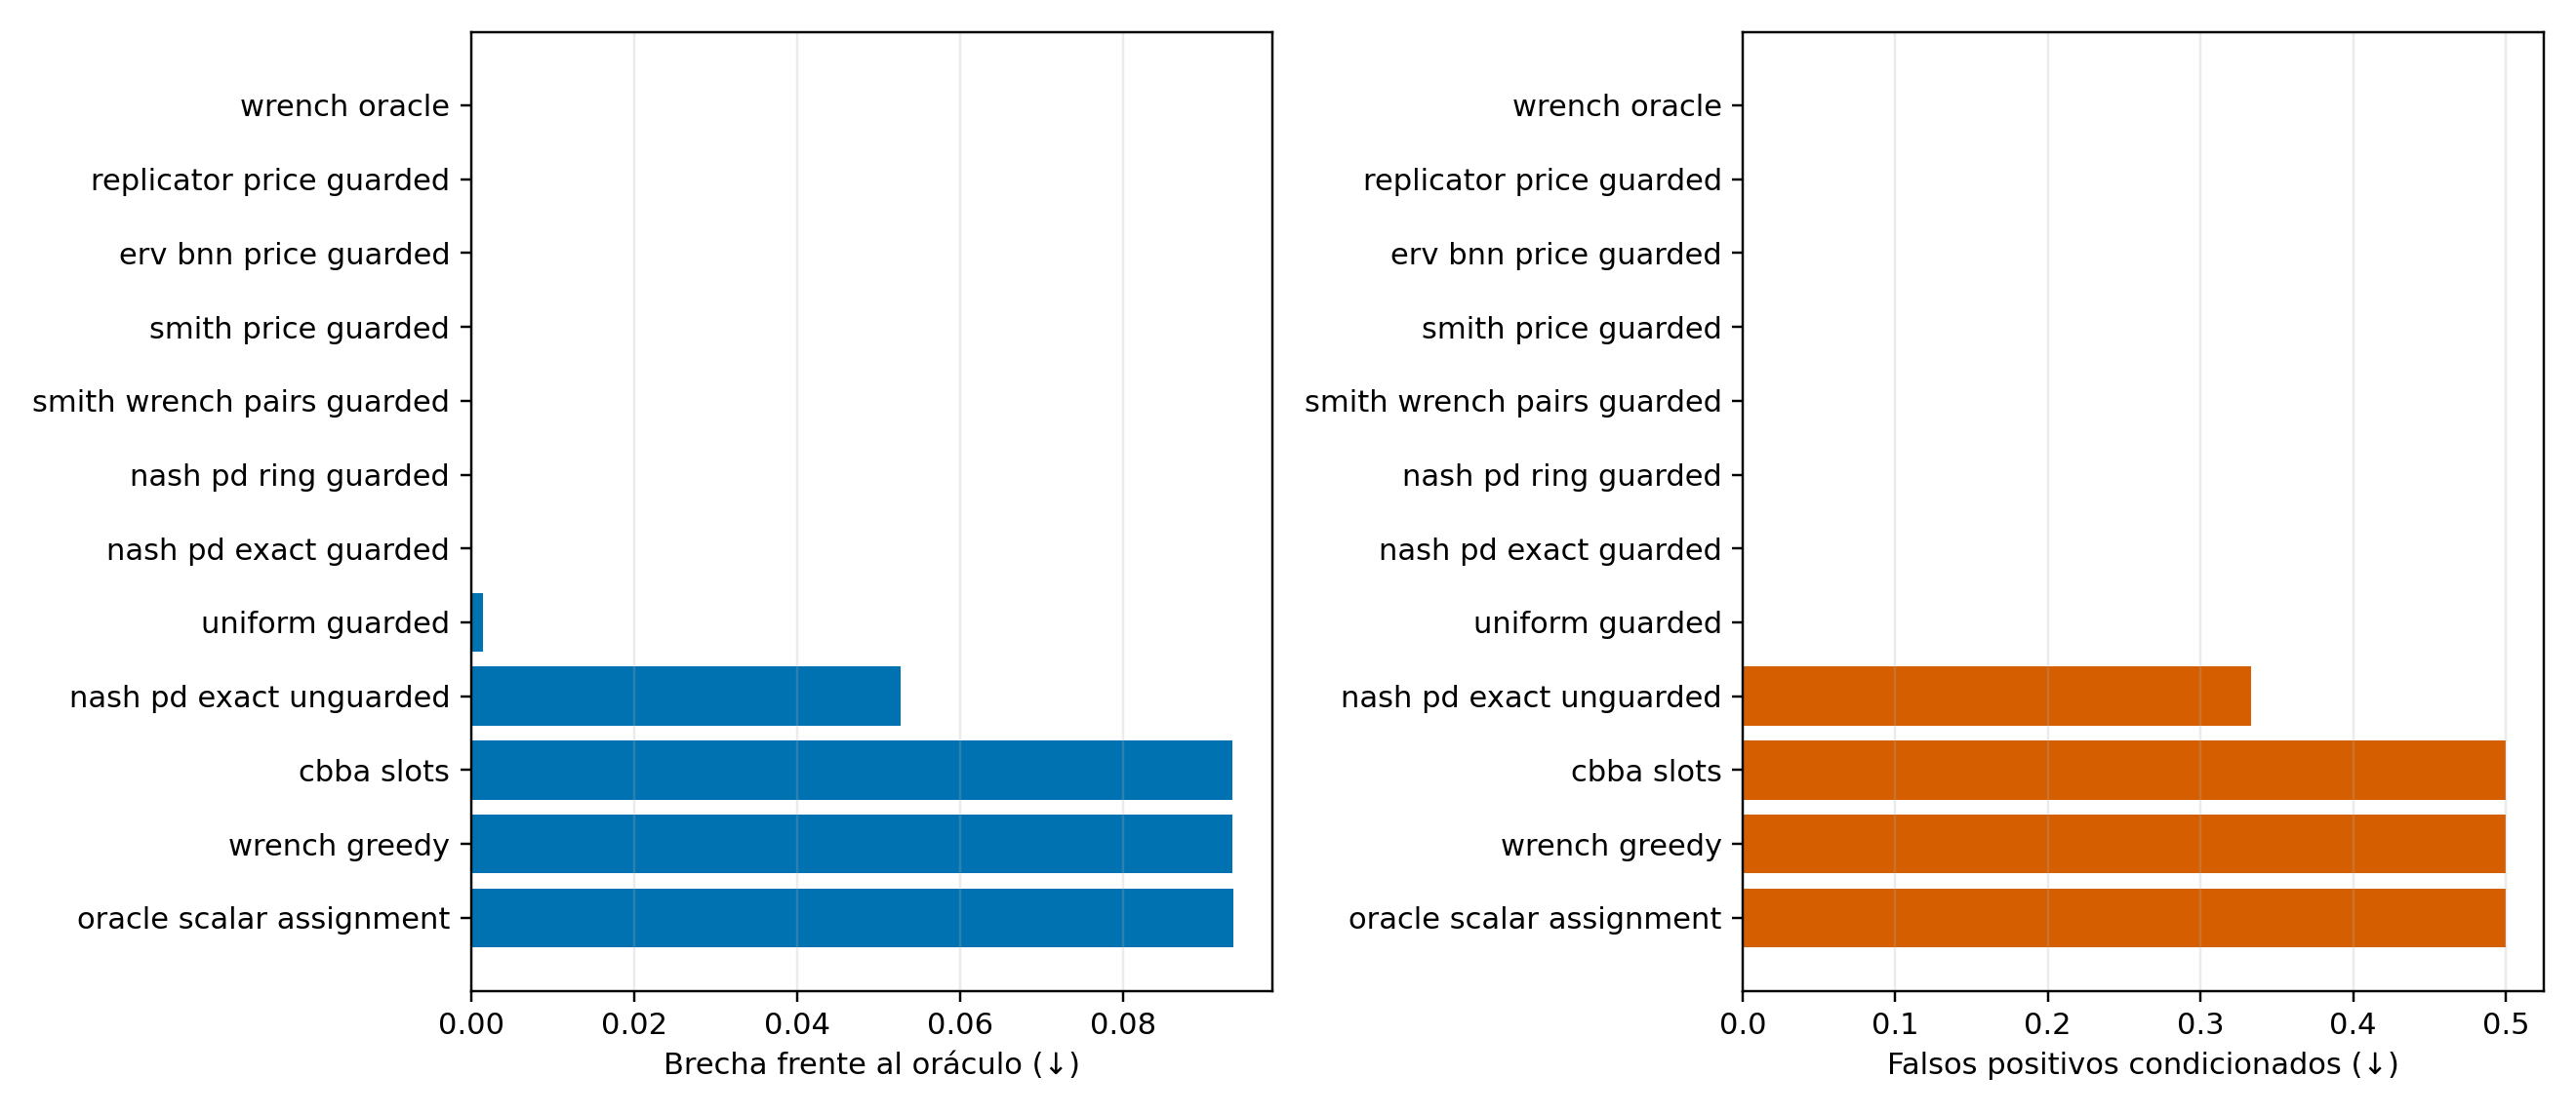
\includegraphics[width=\textwidth]{figures/fig-sp3-wrench-game-performance.png}
\caption[Rendimiento y falsos positivos de SP3]{Brecha respecto del oráculo y falsos positivos condicionados por método.}
\viuownsource
\label{fig:sp3-wrench-game-performance}
\end{figure}

\subsubsection{Resultados confirmatorios}

La auditoría v1.1 terminó en PASS. En 3600 ejecuciones de juego, el error máximo del
simplex fue $4{,}44\times10^{-16}$. Projected primal--dual exacto obtuvo brecha máxima
de potencial $0{,}00339$ frente al QP y violación máxima de slots $0{,}00467$.
Las 600 referencias QP auditadas convergieron y ninguna variante guardada produjo
falsos positivos.

\begin{table}[H]
\centering
\caption{Resultados canónicos de SP3 v1.1. Menor FP y brecha es mejor.}
\label{tab:sp3-v11-main}
\scriptsize
\begin{tabular}{@{}lrrrrr@{}}
\toprule
Método & Cobertura & Precisión & FP & Brecha & Tiempo (s)\\
\midrule
Oráculo wrench & 1,0000 & 1,0000 & 0,0000 & 0,0000 & 0,1179\\
PD exacto+guardia & 1,0000 & 1,0000 & 0,0000 & 0,0002 & 0,3021\\
PD anillo+guardia & 1,0000 & 1,0000 & 0,0000 & 0,0001 & 0,4710\\
Smith precio+guardia & 1,0000 & 1,0000 & 0,0000 & 0,0000 & 0,2362\\
Replicator precio+guardia & 1,0000 & 1,0000 & 0,0000 & 0,0000 & 0,1569\\
ERV--BNN precio+guardia & 1,0000 & 1,0000 & 0,0000 & 0,0000 & 0,1861\\
Pareado+guardia & 1,0000 & 1,0000 & 0,0000 & 0,0000 & 0,1406\\
Uniforme+guardia & 1,0000 & 1,0000 & 0,0000 & 0,0015 & 0,0598\\
PD exacto sin guardia & 1,0000 & 0,6667 & 0,3333 & 0,0527 & 0,3021\\
CBBA slots & 1,0000 & 0,5000 & 0,5000 & 0,0933 & 0,0239\\
Greedy wrench & 1,0000 & 0,5000 & 0,5000 & 0,0934 & 0,0237\\
Oráculo escalar & 1,0000 & 0,5000 & 0,5000 & 0,0935 & 0,0197\\
\bottomrule
\end{tabular}
\end{table}

La guardia reduce el FP de PD exacto en $-0{,}3333$
(IC95\,\% $[-0{,}3700,-0{,}2950]$, $p_{\rm Holm}<10^{-34}$). PD
guardado reduce la brecha frente al escalar en $-0{,}0933$; el cierre pareado reduce
la de CBBA en $-0{,}0933$; ambos sobreviven Holm. La información exacta reduce el
residual KKT frente al anillo en $-0{,}0181$
(IC95\,\% $[-0{,}0201,-0{,}0162]$, $p_{\rm Holm}<10^{-90}$).

\begin{figure}[H]
\centering
\begin{minipage}[t]{0.49\textwidth}
\centering
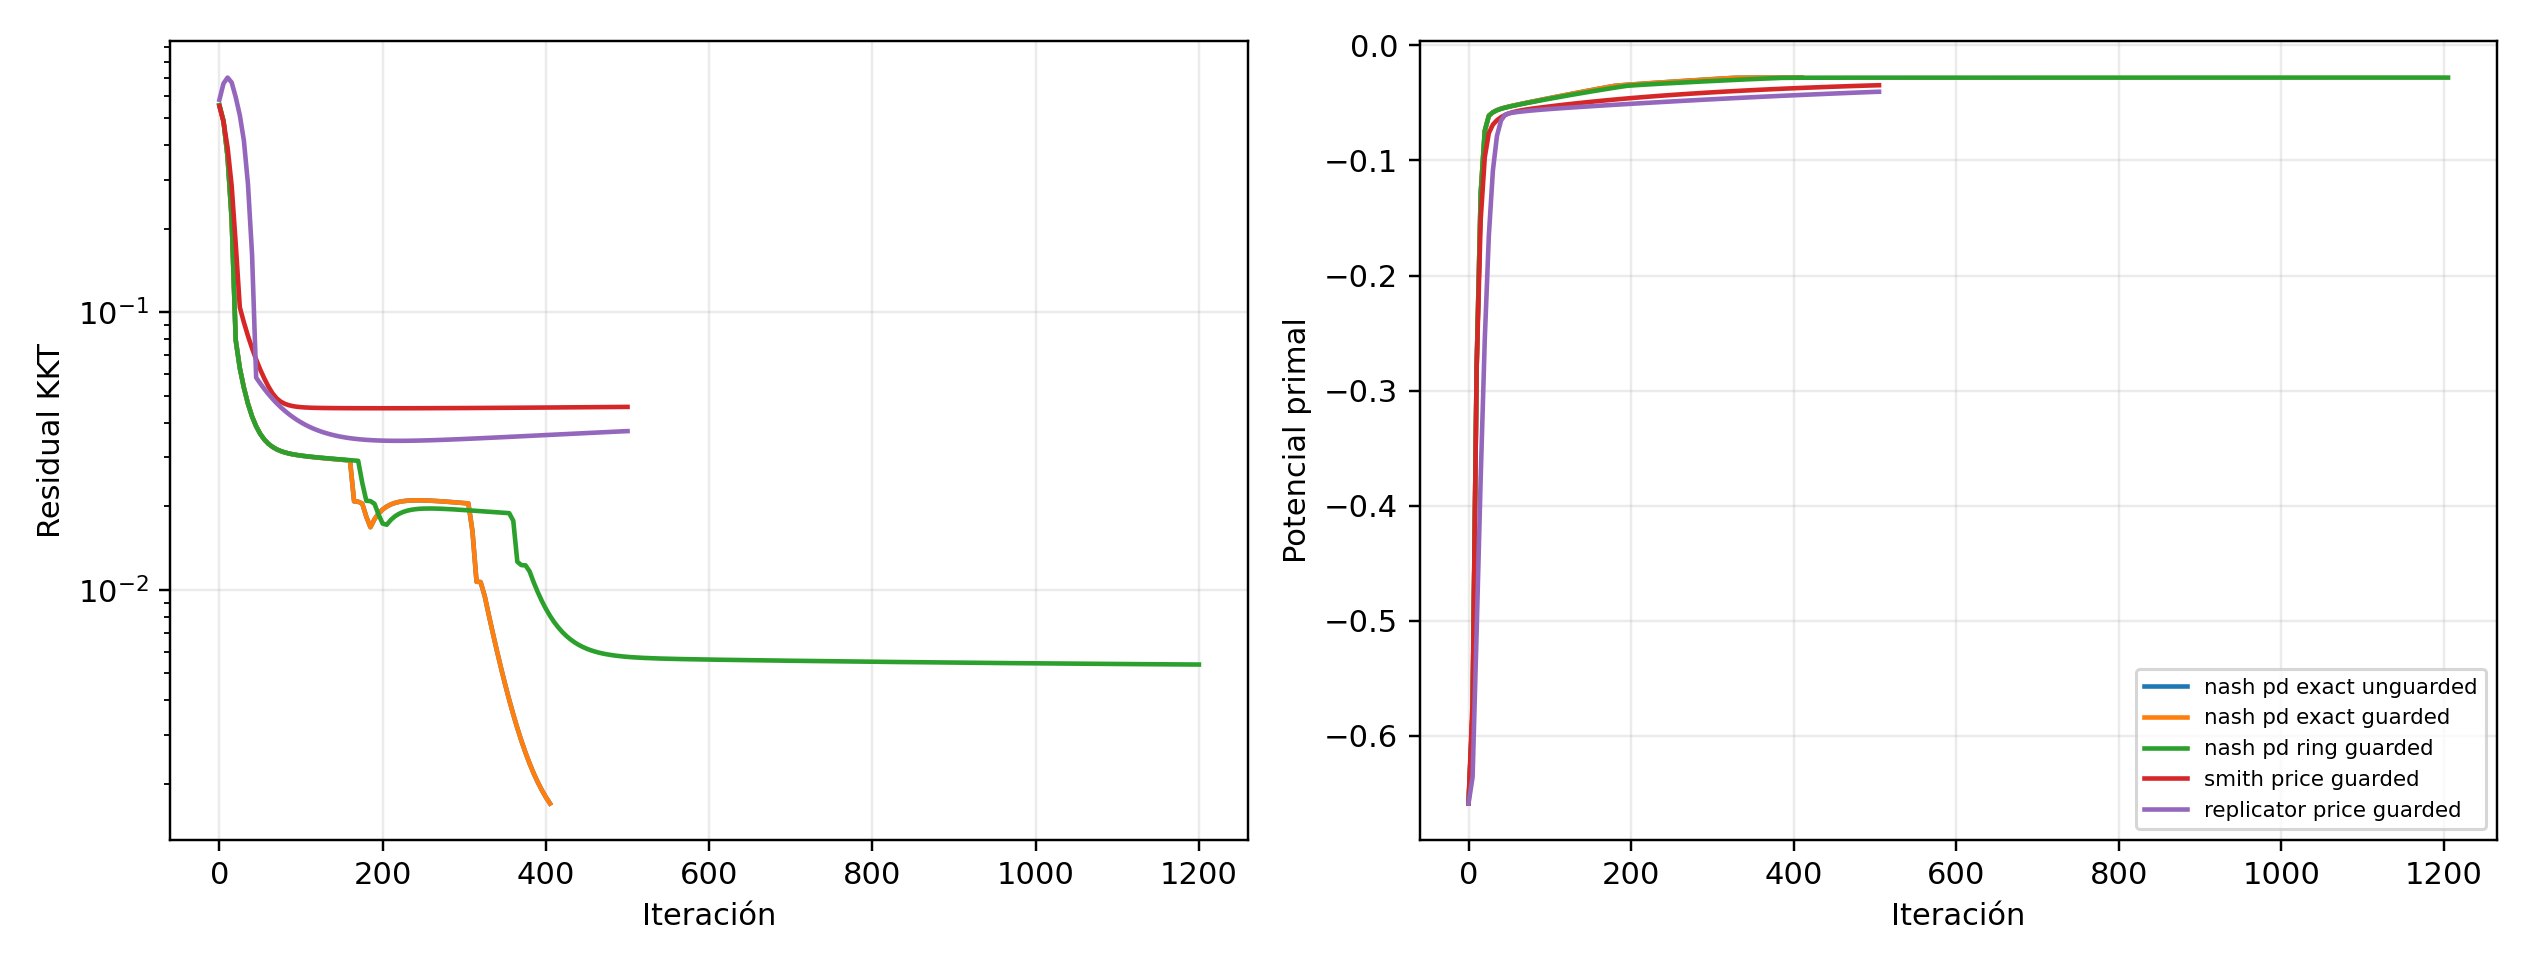
\includegraphics[width=\linewidth]{figures/fig-sp3-kkt-potential.png}
\end{minipage}\hfill
\begin{minipage}[t]{0.49\textwidth}
\centering
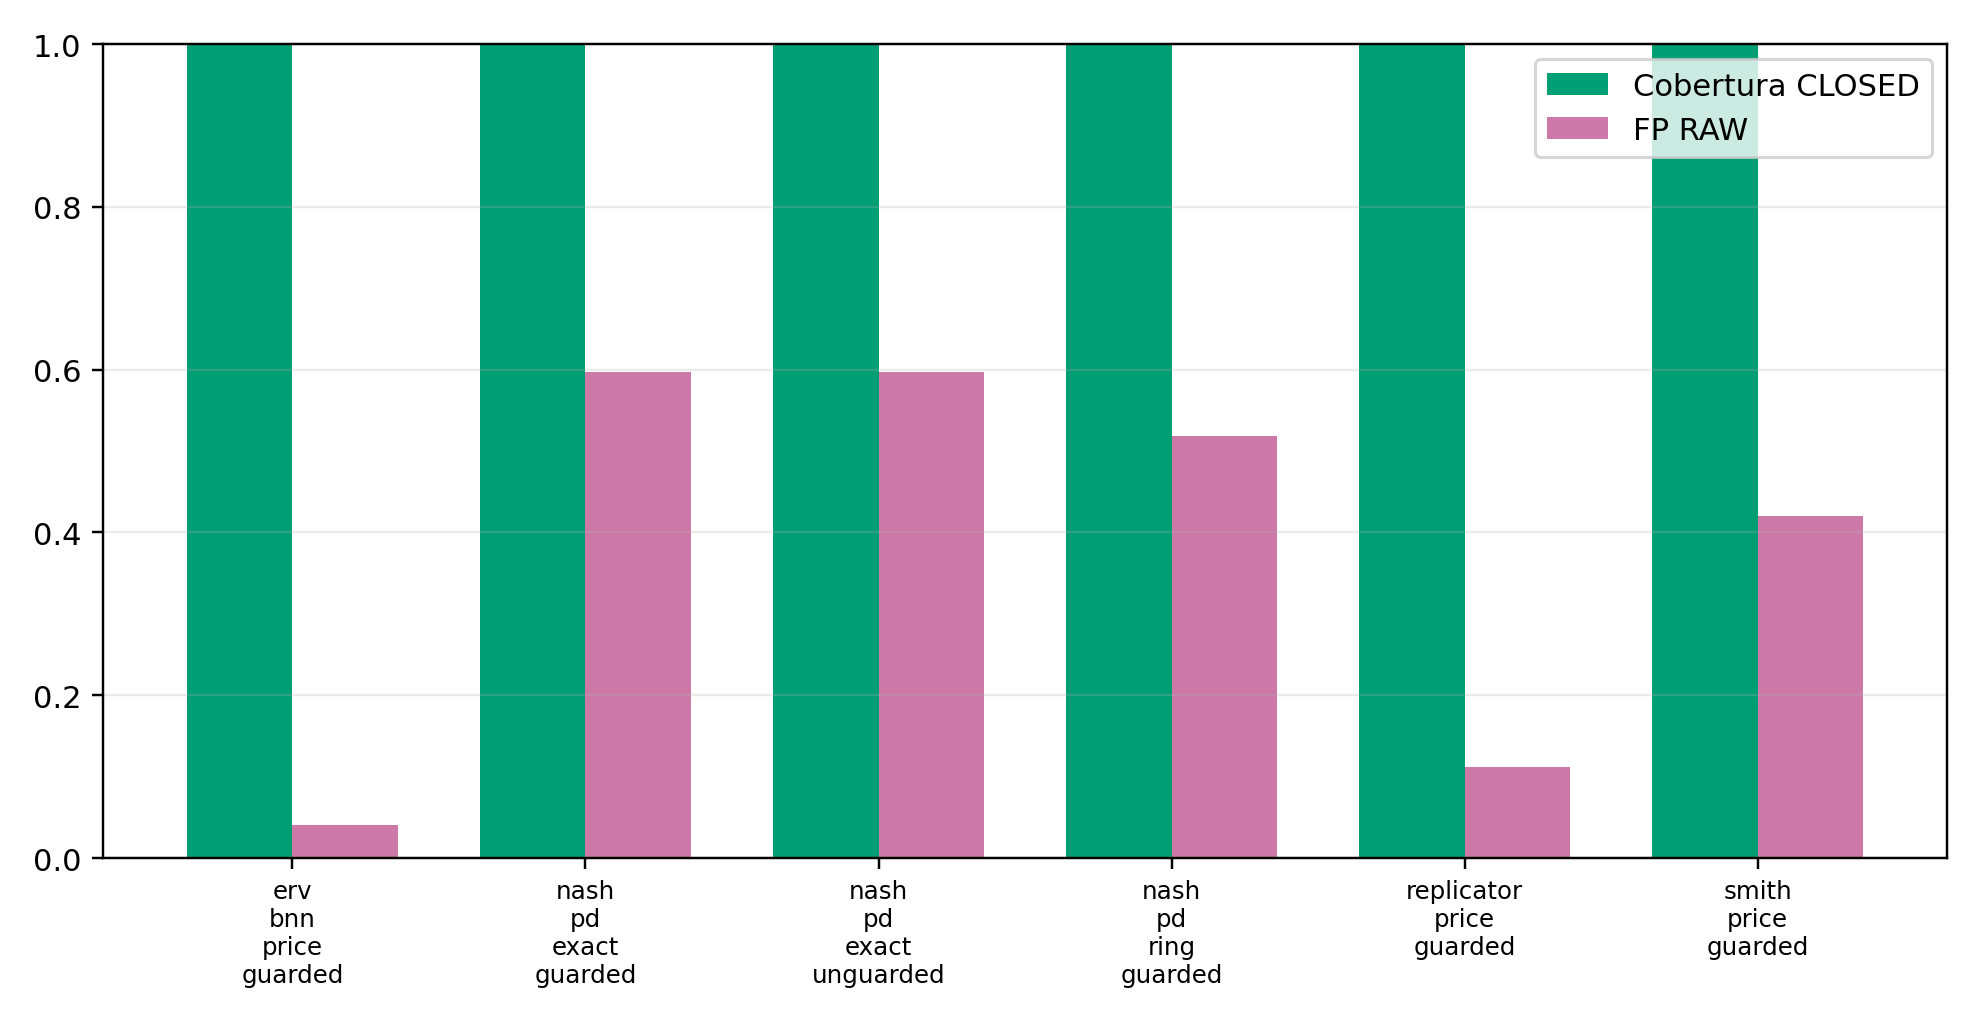
\includegraphics[width=\linewidth]{figures/fig-sp3-protocol-closure.png}
\end{minipage}
\caption[Convergencia y ablación del cierre en SP3]{Residual KKT/potencial y separación entre desempeño RAW y CLOSED.}
\viuownsource
\label{fig:sp3-kkt-closure}
\end{figure}

La lectura RAW impide atribuir todo el resultado al juego. PD exacto presenta FP RAW
$0{,}5967$ y solo $0{,}1508$ de cargas wrench-factibles; después del cierre de slots,
pero sin guardia, conserva FP $0{,}3333$. Smith, replicator y BNN tienen FP RAW
$0{,}4208$, $0{,}1117$ y $0{,}0400$, pero los dos últimos no completan cargas en RAW.
La guardia transforma todas estas preferencias en cobertura $1$. Además,
uniforme+guardia también alcanza cobertura $1$ y brecha $0{,}0015$.

\paragraph{Aporte y límite de SP3.}
SP3 demuestra que capacidad escalar y factibilidad wrench son constructos distintos,
formula una relajación como juego potencial con restricciones compartidas, vincula
v-GNE y KKT, implementa Nash seeking con precio residual y verifica un cierre que
elimina falsos positivos dentro del modelo planar. No demuestra superioridad del motor
poblacional ni distribución extremo a extremo: la guardia global domina el resultado
CLOSED y los escenarios tienen hasta ocho robots y dos cargas. Tampoco demuestra
fricción tridimensional, deformación, deslizamiento ni seguridad física. La extensión
prioritaria es reemplazar la reparación global por clearing pareado distribuido y
validarlo con grafos variables y contacto físico.
